\section{Mikrocontroller}\label{Appendix:Mikrocontroller}


\subsection{Inbetriebnahme}\label{Appendix:Inbetriebnahme_uC}

\subsubsection{Fuse-Bits}

%\begin{table}[h!]
%\center
%\begin{tabular}{|l|l|l|l|l|}
%\hline
%Bit & Register-Name & Default & Programmed & Mixer (0xFF)\\ \hline
%0 & BODLEVEL0 & 1 & 0 (1.8V) & 1\\
%1 & BODLEVEL1 & 1 & 0 (2.7V) & 1\\
%2 & BODLEVEL2 & 1 & 0 (4.3V) & 1\\
%3 & - & 1 & - & 1 \\
%4 & - & 1 & - & 1 \\
%5 & - & 1 & - & 1 \\
%6 & - & 1 & - & 1 \\
%7 & - & 1 & - & 1 \\ \hline
%\end{tabular}
%\label{tab:Extended_Fuses}
%\caption{Bits Etended Fuses.}
%\end{table}

%\begin{tabularx}{\textwidth}{ll|X}
%
%BODLEVEL0:2 				& : 	& Setzt die Brown-Out-Spannung. Sobald die Versorgungsspannung unterdiese Schwelle fällt, schaltet der uC aus. Für: 
%\begin{tabular}{lll}
%1.8V 		& = & 0b11111110\\
%2.7V 		& = & 0b11111101\\
%4.5V 		& = & 0b11111011\\
%disabled 	& = & 0b11111111
%\end{tabular}
%
%%\todo{cite: Atmel Datenblatt Seite 48}\\
%
%\end{tabularx}
%\todo{cite: Siehe Cites auskommentiert in Tabelle}

%\begin{table}[h!]
%\center
%\begin{tabular}{|l|l|l|l|l|l|l|l|l|}
%\hline
%Bit & Register-Name 	& Default 	& Programmed 							& Mixer (0xD0)\\ \hline
%0 	& BOOTRST  		& 1 			& 0 (Startet Bootloader bei Reset) 		& 0\\
%1 	& BOOTSZ0  		& 0 			& X (Definiert Bootloader-Speicherplatz) 	& 0\\
%2 	& BOOTSZ1  		& 0 			& X (Definiert Bootloader-Speicherplatz) 	& 0\\
%3 	& EESAVE  		& 1 			& 0 (Schützt EEPROM während Löschen) 	& 0\\
%4 	& WDTON 			& 1 			& 0 (Watchdog immer Ein)					& 1\\
%5 	& SPIEN 			& 0 			& 0 (Aktiviert ISP-Schnittstelle)		& 0\\
%6 	& JTAGEN 		& 0 			& 0 (Aktiviert JTAG-Schnittstelle) 		& 1\\
%7 	& OCDEN 			& 1 			& 0 (z.T Clock in Sleep-Modus) 			& 1\\ \hline
%\end{tabular}
%\label{tab:High_Byte_Fuses}
%\caption{Bits High-Byte-Fuses.}
%\end{table}

Da während dem Entwickeln die Möglichkeit bestehen soll, den Flash-Speicher per USB zu beschreiben, muss beim Aufstarten der BL aufgerufen werden. Dazu muss das BOOTRST-Bit aktiviert werden. Der Speicherplatz für den BL wird auf 4096 words gesetzt. Das EEPROM soll beim Löschen des \textmu C geschützt bleiben, weshalb das EESAVE-Bit aktiviert wird. Da die ISP-Schnittstelle benötigt wird, um den BL zu schreiben und Fuse-Bits zu setzen, wird das SPIEN-Bit gesetzt.
%
%\begin{tabularx}{\textwidth}{ll|X}
%
%BOOTRST 	& : 	& 
%Nach Reset wird Programm von Bootloader-Memory-Section gestartet. Wenn ein Bootloader verwendet wird, um den Mikrocontroller zu flashen, muss dieses Bit aktiviert sein. \\ \hline
%
%%\todo{cite: https://embedds.com/all-you-need-to-know-about-avr-fuses/}\\
%
%BOOTSZ0:1 		& : &
%Definiert Bootloader-Grösse (je kleiner desto mehr Platz für Applikation). Grössen : 512, 1024,2048,4096 words.\\ \hline
%
%%\todo{cite: Atmel Datenblatt Seite 320}\\
%
%EESAVE 				& : & 
%Schütz EEPROM-Speicher währenddem der Chip gelöscht wird.\\ \hline
%
%%\todo{cite: https://embedds.com/all-you-need-to-know-about-avr-fuses/}\\
%
%
%WDON 				& : & 
%Forciert Chip-Reset, wenn nichts spezielles passiert.\\ \hline
%
%%\todo{cite: https://embedds.com/all-you-need-to-know-about-avr-fuses/}\\
%
%SPIEN 				& : & 
%Aktiviert die ISP-Schnittstelle. Don't touch!\\ \hline
%
%%\todo{cite: https://www.mikrocontroller.net/articles/AVR\_Fuses}\\
%
%JTAGEN 				& : & 
%Aktiviert die JTAG-Schnittstellt. Wird empfohlen auszuschalten wenn nicht benötigt.\\ \hline
%
%%\todo{cite: https://www.mikrocontroller.net/articles/AVR\_Fuses}\\
%
%OCDEN 				& : & 
%Ermöglicht gewissen Teilen des Clock-Systems während eines sleep-modus weiterhin zu laufen.\\
%
%%\todo{cite: Atmega2560 Datenblatt, Seite 327}\\
%
%\end{tabularx}
%\todo{cite: Siehe Cites auskommentiert in Tabelle}
%
%\begin{table}[h!]
%\center
%\begin{tabular}{|l|l|l|l|l|l|l|l|l|}
%\hline
%Bit & Register-Name 	& Default 	& Programmed 						& Mixer (0xF7)\\ \hline
%0 	& CKDIV8 		& 0 			& 0 (System-Clock-Prescaler = 8)		& 0\\
%1 	& CKOUT  		& 1 			& 0 (PE7 als System-Clock-Output) 	& 1\\
%2 	& SUT1			& 1 			& X (Aufstartzeit) 					& 0\\
%3 	& SUT0			& 0 			& X (Aufstartzeit) 					& 0\\
%4 	& CKSEL3			& 0 			& X (Frequenzbereich)				& 1\\
%5 	& CKSEL2			& 0 			& X (Frequenzbereich)				& 1\\
%6 	& CKSEL1			& 1 			& X (Frequenzbereich)				& 1\\
%7 	& CKSEL0			& 0 			& X (Aufstartzeit)					& 0\\
%\hline
%\end{tabular}
%\label{tab:Low_Byte_Fuses}
%\caption{Bits Low-Byte-Fuses.}
%\end{table}
%
Für den Mikrocontroller verwenden wir einen 16MHz Full-Swing-Crystal-Oszillator, weshalb die Bits CKSEL3:1 auf 111 stehen müssen.
Die Aufstartzeit wird vorsorglich auf die längst mögliche Zeit eingestellt. Dies führt dazu, dass das Register CKSEL0 auf 0 und die Register SUT0:1 auf 00 gesetzt werden.
%
%
%\begin{tabularx}{\textwidth}{ll|X}
%
%CKDIV8 				& : 	& Setzt den Initialwert des System-Clock-Prescalers auf 8.
%\\ \hline
%
%%\todo{cite: Atmel Datenblatt Seite 48}\\
%
%CKOUT 				& : & Setzt den Pin PE7 als System-Clock-Output.
%\\ \hline
%
%%\todo{cite: Atmega Datenblatt Seite 327}\\
%
%SUT0:1 				& : & Setzt Parameter zur Aufstartzeit.
%\\ \hline
%
%%\todo{cite: Atmel Datenblatt Seite 42}\\
%
%CKSEL0:3 			& : & Setzt Parameter zum Oszillator (CKSEL1:3) und Aufstartzeit (CKSEL0).
%\\ \hline
%
%%\todo{cite: Atmel Datenblatt Seite 42}\\
%
%\end{tabularx}
%\todo{cite: Siehe Cites auskommentiert in Tabelle}
%
Der Brown-out-Detektor setzt den internen Reset, sobald die Versorgungsspannung unter einen Wert fällt. Wenn der Mikrocontroller ausfällt, während der TMC4671 noch aktiv ist, wird der Motor weiter gefahren. Dieses Risiko soll eingeschränkt werden, indem dieser Modus ausgeschaltet wird.\cite{haftmann_programmierung_nodate}

%\subsubsection{Brown-out-Detection}\label{Appendix:Brown-out-Detection}

\begin{figure}[H]
	\centering
	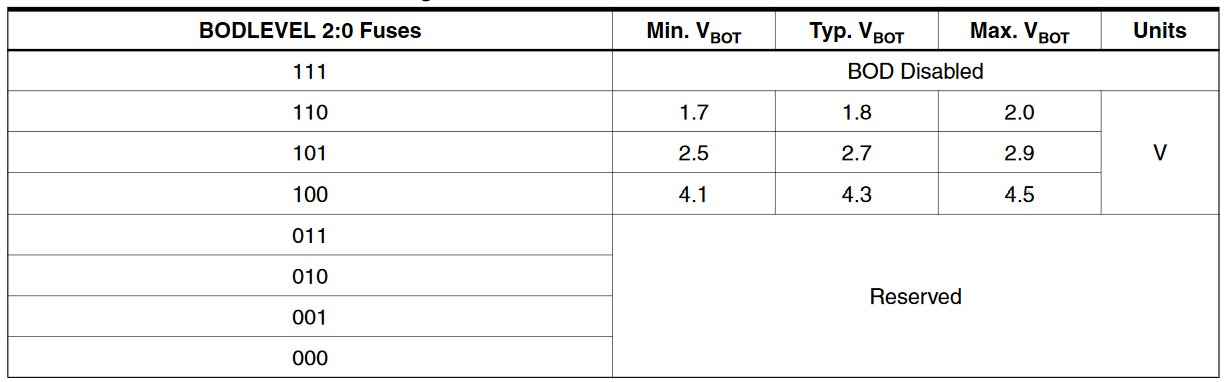
\includegraphics[width=0.7\textwidth]{graphics/Tabelle_BoD}
	\caption{Tabelle Brown-out-Detection.\cite[S.361]{atmel_atmel_2014}}
	\label{fig:Tabelle_BoD}
\end{figure}

%\subsubsection{Full Swing Crystal Oscillator}\label{Appendix:Full_Swing _Crystal_Oscillator}

\begin{figure}[H]
	\centering
	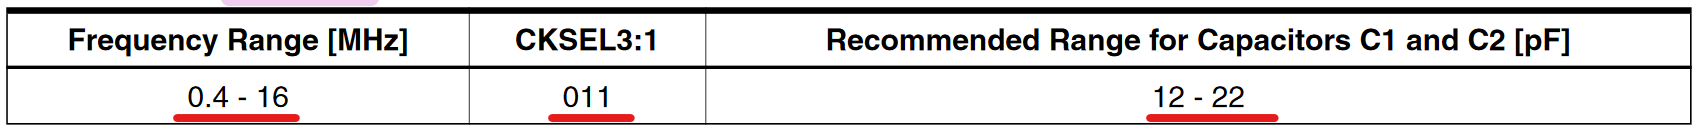
\includegraphics[width=0.7\textwidth]{graphics/Tabelle_Crystal}
	\caption{Tabelle Frequenzbereich Crystal Oszillator.\cite[S.43]{atmel_atmel_2014}}
	\label{fig:Tabelle_Crystal}
\end{figure}

\begin{figure}[H]
	\centering
	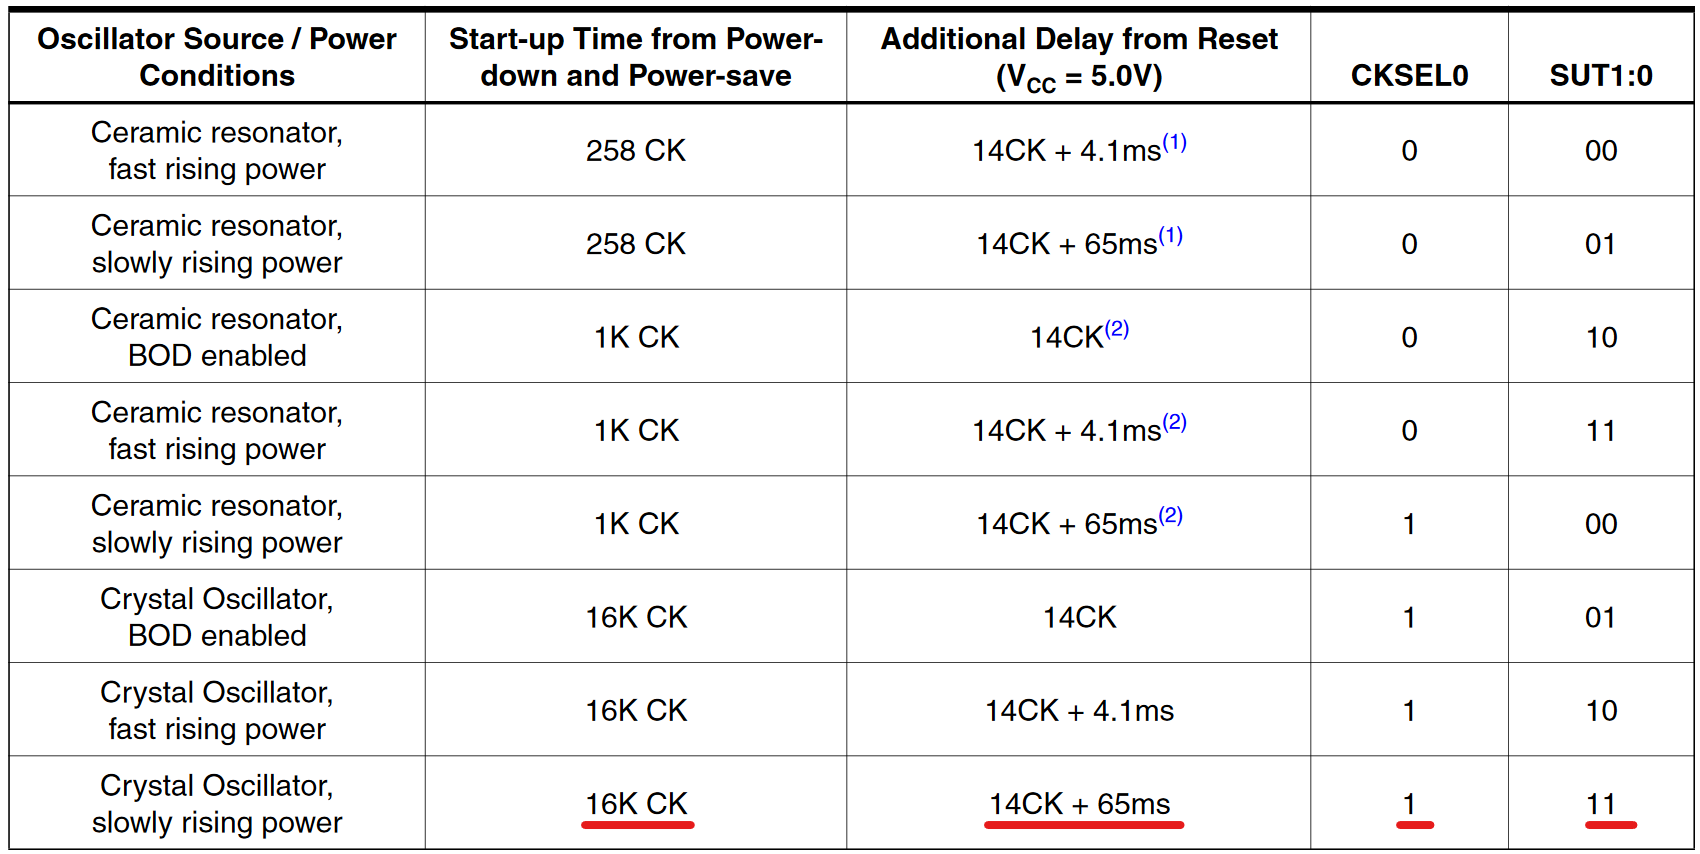
\includegraphics[width=0.7\textwidth]{graphics/Tabelle_Crystal2}
	\caption{Tabelle Aufstartzeit.\cite[S.43]{atmel_atmel_2014}}
	\label{fig:Tabelle_Crystal2}
\end{figure}

%\subsubsection{Bootloader-Speicherplatz}\label{Appendix:Bootloader-Speicherplatz}

\begin{figure}[H]
	\centering
	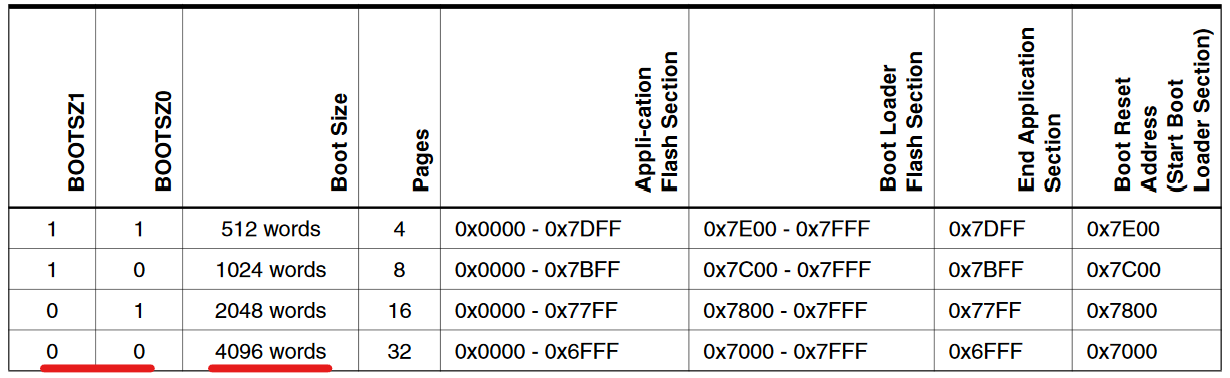
\includegraphics[width=0.7\textwidth]{graphics/Tabelle_Bootloader}
	\caption{Tabelle Bootloader Speicherplatz.\cite[S.320]{atmel_atmel_2014}}
	\label{fig:Tabelle_Bootloader}
\end{figure}

\begin{figure}[H]
	\centering
	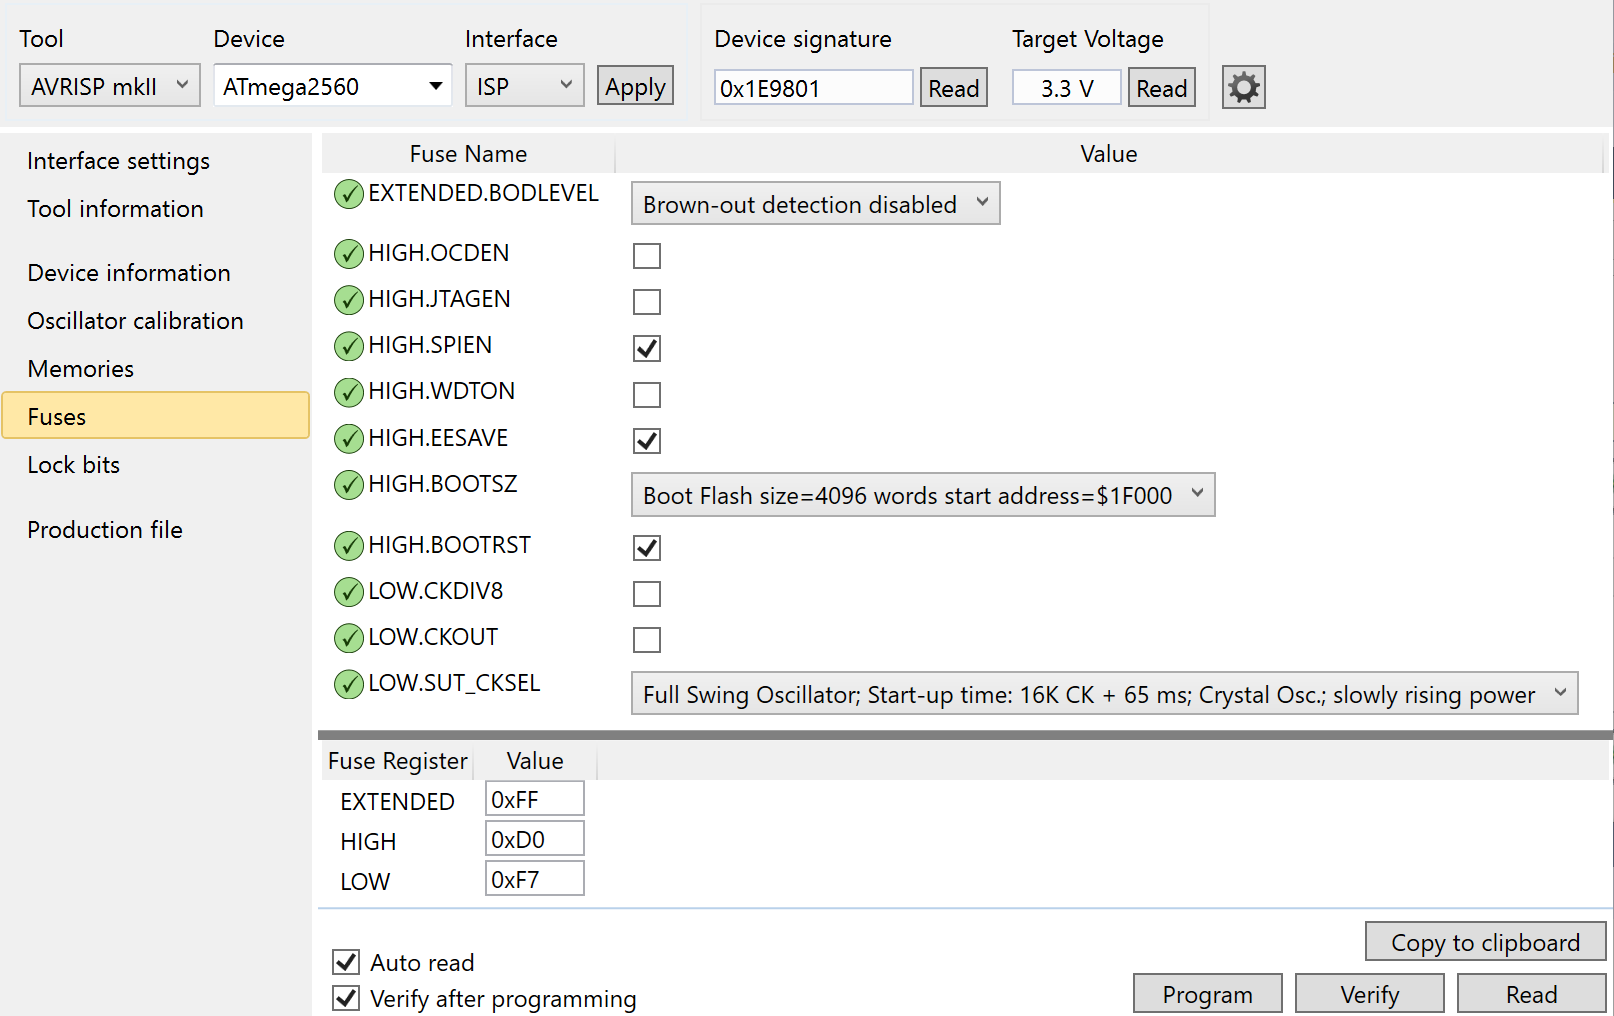
\includegraphics[width=\textwidth]{graphics/AtmelStudio_Fuses}
	\caption{Fuse-Bits Atmega2560 (Atmel Studio).}
	\label{fig:AtmelStudio_Fuses}
\end{figure}

\subsubsection{Bootloader}\label{Appendix:Inbetriebnahme_Bootloader}

Ein Bootloader (BL) ermöglicht seitens Mikrocontroller den Programmiervorgang über USB und stellt sicher, dass der frisch kompilierte Code in den Programmspeicher des Mikrocontrollers gelangt. Im Grunde ist der BL ein Code am Beginn des Programmablaufs, welcher entsprechend nach einem Reset aufgerufen wird. Innerhalb des BL-Codes wird für zwei Sekunden auf eingehende Daten der UART0-Schnittstelle gewartet.
%Wenn innerhalb von ca. zwei Sekunden keine Daten ankommen, wird das Anwenderprogramm gestartet. 
Wird innerhalb dieser zwei Sekunden ein Anwenderprogramm in Form eines HEX-Files an den Mikrocontroller gesendet, wird es gemäss stk500v2-Protokoll in den Flash-Speicher geladen.
%Nach dem Laden in den Flash-Speicher wird das neu geladene Programm gestartet. 
Aufgrund des BL geht es nach einem Reset des \textmu Cs zwei Sekunden, bis das eigentliche Programm startet. \cite{atmel_avr068_2006}

Für den \textmu C des Partymixers wird ein stk500v2-BL verwendet. Dieser kann bei Github heruntergeladen werden \cite{sproul_arduinoarduino-stk500v2-bootloader_2012}. Im File stk500v2.c befinden sich einige Anweisungen, welche Fuse- und Lock-Bits wann gesetzt werden müssen. Durch Anpassen des Startvektors auf den Programmspeicher und Setzen der korrekten Bootloader-Fuses wäre es möglich, den BL-Speicherplatz zu verkleinern um den Programmspeicher zu vergrössern. Dies ist jedoch nicht Inhalt dieses Projektes.

%Wie der Flash-Speicher grob organisiert ist wird in Abbildung \ref{fig:Flash_Speicher_uC} gezeicht. Der Flash-Speicher für den Bootloader, wird in eine No-Read-While-Write Section geschrieben. Das Anwendungsprogramm in die Read-While-Write Section.

%\begin{figure}[h!]
%	\centering
%	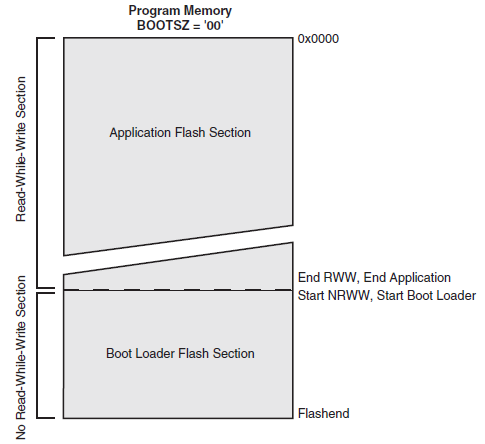
\includegraphics[width=0.8\textwidth]{graphics/Flash_Speicher_uC}
%	\caption{Flas-Speicher Mikrocontroller.}
%	\label{fig:Flash_Speicher_uC}
%\end{figure}
%\todo{cite: https://www.mikrocontroller.net/articles/AVR\_Bootloader\_in\_C\_-\_eine\_einfache\_Anleitung}

\begin{figure}[H]
	\centering
	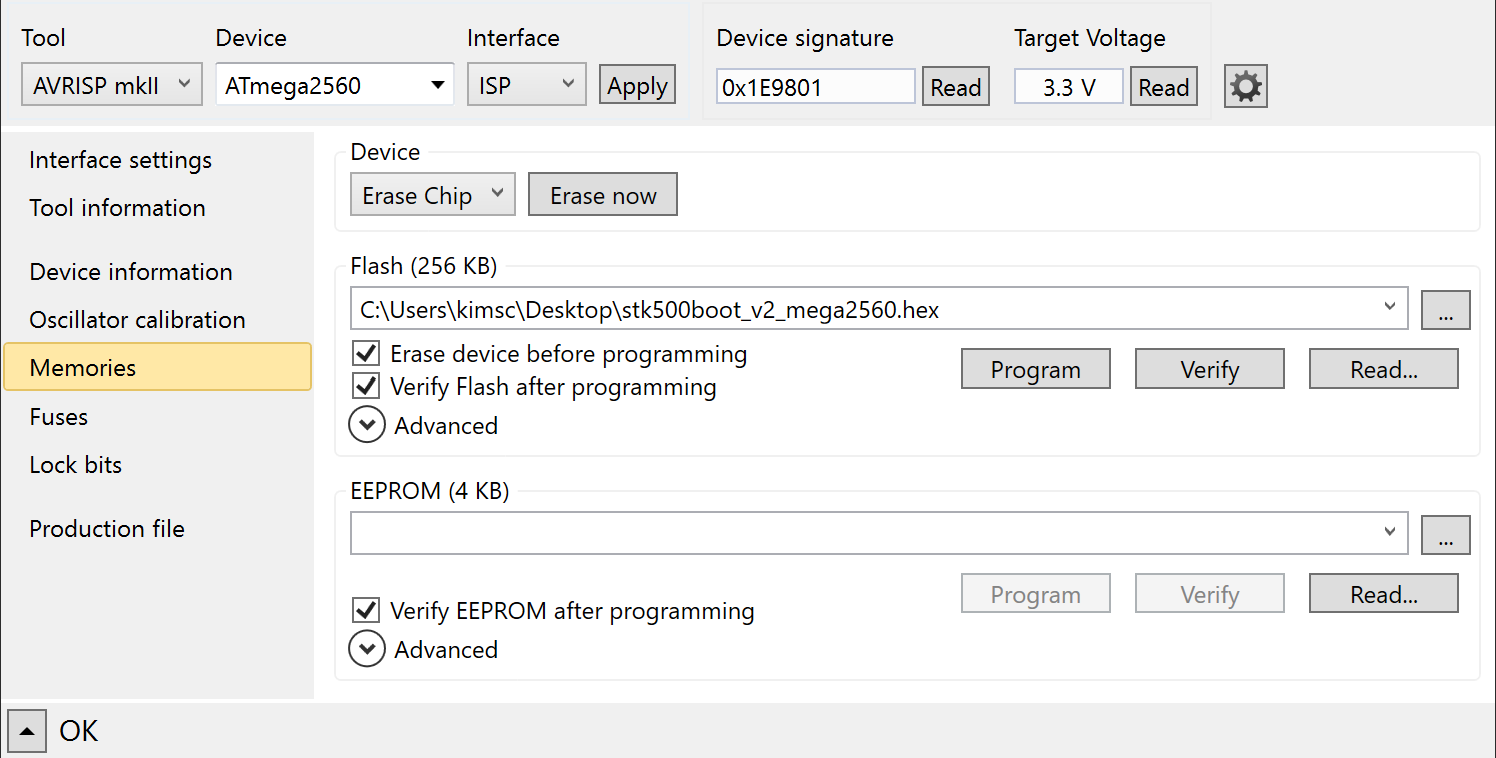
\includegraphics[width=\textwidth]{graphics/AtmelStudio_Program_Bootloader}
	\caption{Bootloader brennen (Atmel Studio).}
	\label{fig:AtmelStudio_Program_Bootloader}
\end{figure}

\subsubsection{Lock-Bits}

Die Lock-Bits müssen gesetzt werden, nachdem der BL in den Speicher geschrieben wurde. ''SPM ist nicht erlaubt, in den Anwenderbereich zu schreiben und LPM ist nicht erlaubt aus dem Applikationssktor zu lesen, wenn LPM aus dem Urlader-Bereich ausgeführt wird.''\cite{haftmann_programmierung_nodate}

%\subsubsection{Memory-Lock Bootloader}

\begin{figure}[H]
	\centering
	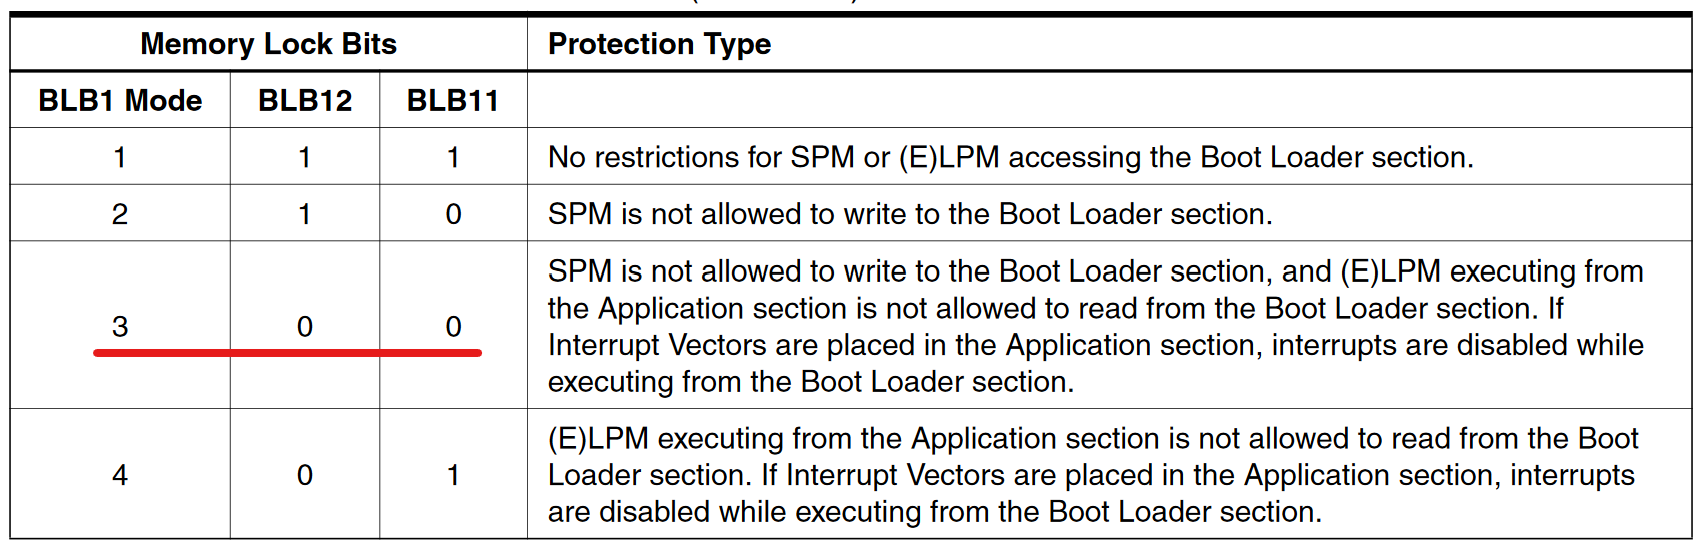
\includegraphics[width=0.7\textwidth]{graphics/Tabelle_Memory_Lock}
	\caption{Tabelle Memory Lock.\cite[S.326]{atmel_atmel_2014}}
	\label{fig:Tabelle_Memory_Lock}
\end{figure}

\begin{figure}[H]
	\centering
	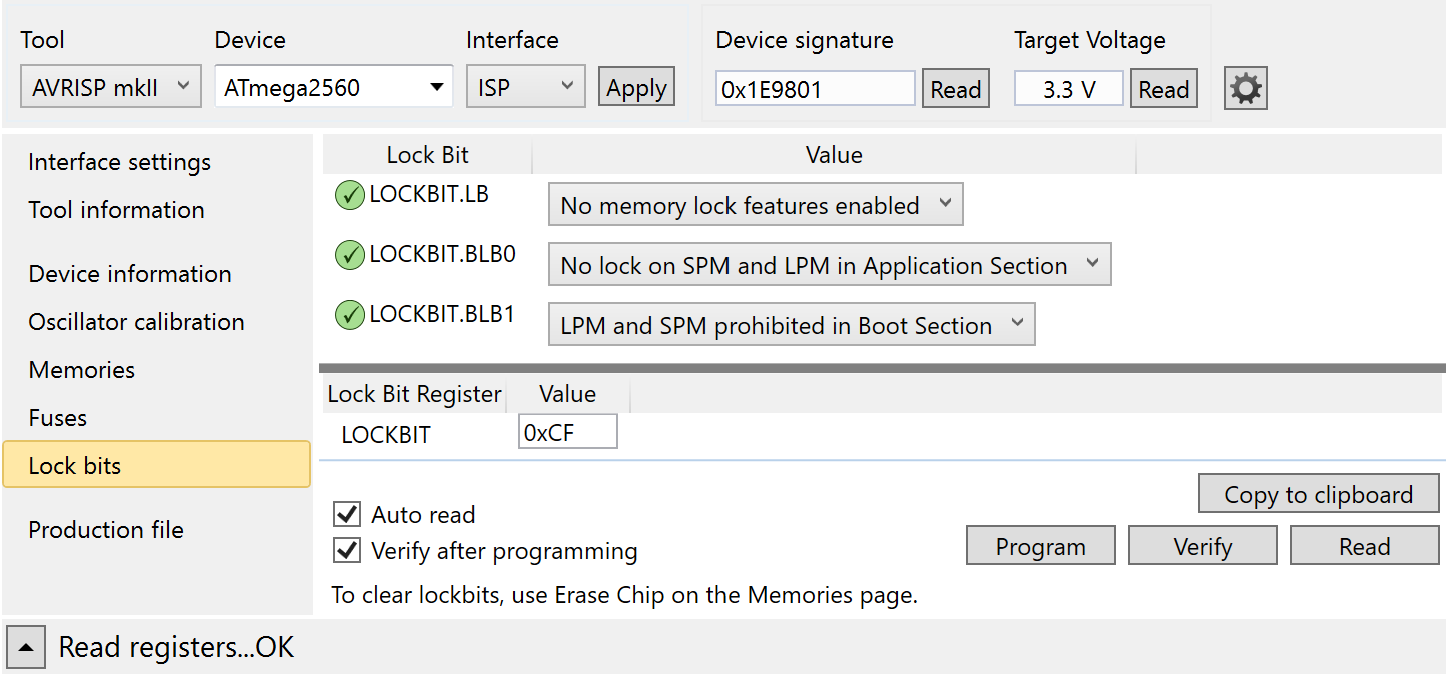
\includegraphics[width=\textwidth]{graphics/AtmelStudio_Locks}
	\caption{Lock-Bits Atmega2560.}
	\label{fig:AtmelStudio_Locks}
\end{figure}


\subsubsection{Einbinden AVRdude und stk500v2 (wiring)}\label{Appendix:AVR_STK500}

\begin{figure}[H]
	\centering
	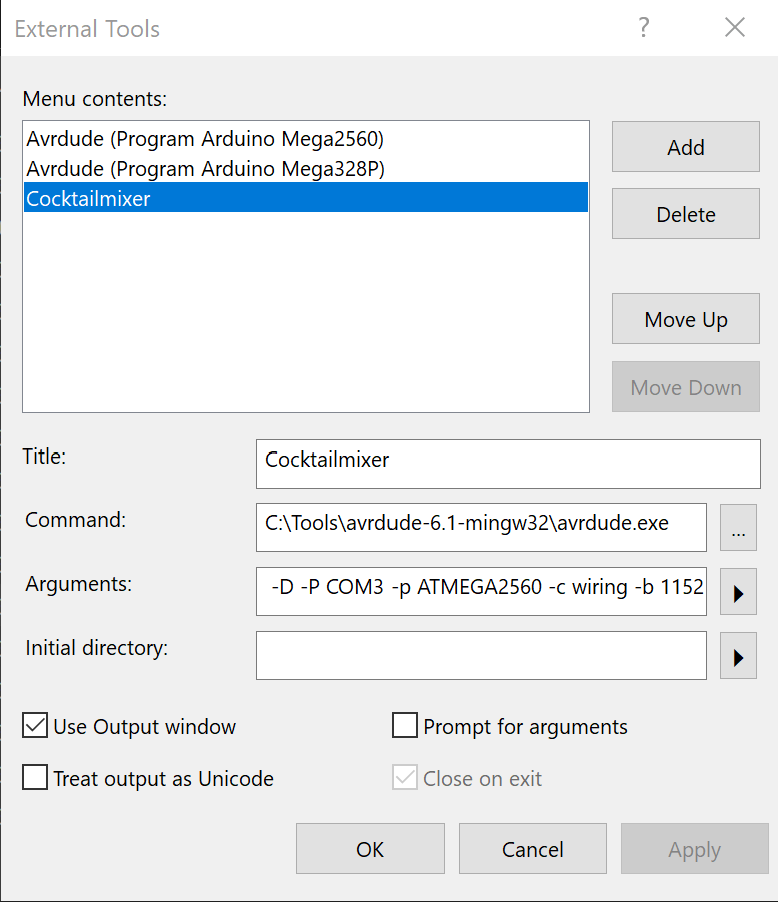
\includegraphics[width=0.5\textwidth]{graphics/AtmelStudio_External_Tools}
	\caption{External Tools Atmega2560 (Atmel Studio).}
	\label{fig:AtmelStudio_External_Tools}
\end{figure}

\subsubsection{Schwingung 16MHz Quarz}

\begin{figure}[H]
\center
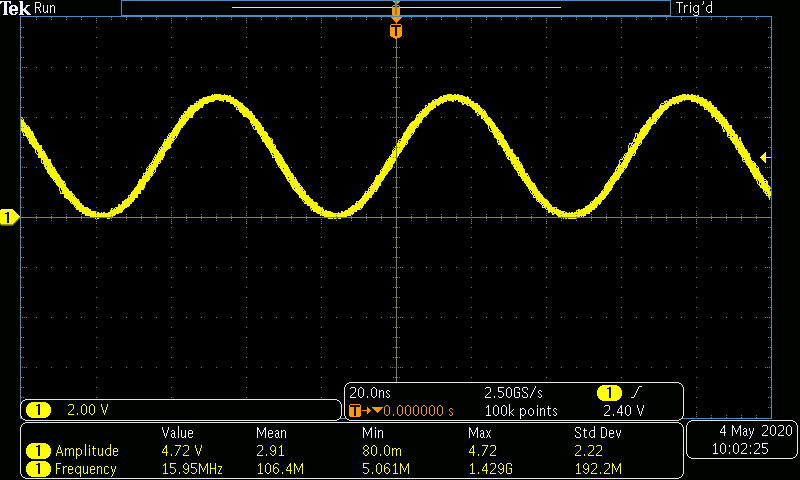
\includegraphics[width = 0.8\textwidth]{graphics/Crystal_Swing}
\caption{Schwingung des Oszillators}
\label{fig:Crystal_Swing}
\end{figure}
